\section{Results}\label{results}
\subsection{MAL effect in the UD collection}\label{results1}
Out of the 186 languages available in our data, we caluclated a $\beta$(1$\rightarrow\infty$) for 131. In these sample we identify 62 languages with a MAL preference, 10 with an Anti MAL preference and 59 in the gray zone. Importantly, these three categories are fairly comparabely well-represented across languages families as well as main syntactic languge types \ref{tab:MAL}).
%For language families, given the unbalanced nature of our sample, we have grouped the languages into the two main Indo-European (IE) and non-Indo-European (non-IE) groups.  

\begin{figure}[!ht]
\begin{center}
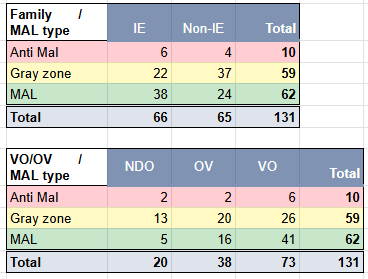
\includegraphics[width=\columnwidth]{latex/MAL.png}
\label{tab:MAL}
\caption{MAL type per language families and VO/OV types.}
\end{center}
\end{figure}

For RMAL (postverbal domain) and LMAL (preverbal domain) we have calculted $\beta$(1$\rightarrow\infty$) for respectively 124 and 103 languages out of the total of 186 languages (Table \ref{tab:HeadR1} and Table \ref{tab:HeadL1})). Interestingly, we find a clear difference between the pre- and postverbal domains. On the one hand, while we identify 62 languages showing a MAL effect, there are 81 languages (79\%) which show a MAL effect in the postverbal domain (or a RMAL effect), against 39 languages (31\%) showing a MAL effect in the preverbal domain (or a LMAL effect). In other words, 79\% of languages show an MAL effect in the postverbal domain, against 31\% in the preverbal domain, while the percentage of languages showing a combined MAL effect is 47\%. On the other hand, while we identify 10 Anti MAL languages, there are 29 Anti LMAL languages and 7 Anti RMAL. In other words, 23\% of languages show an anti MAL effect in the preverbal domain, against 7\% in the postverbal domain, while 8\% show a bilateral anti MAL effect. 

\begin{figure}[!ht]
\begin{center}
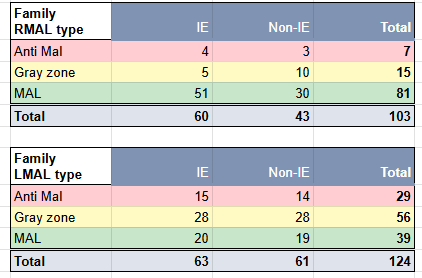
\includegraphics[width=\columnwidth]{latex/FamRL.png}
\label{tab:FamLR}
\caption{RMAL and LMAL per language families.}
\end{center}
\end{figure}

We can hence say that there is both a RMAL and an Anti LMAL bias - in other words, a ference for MAL in the postverbal domain and for Anti MAL in the preverbal domain. Importantly, in our data, like for the combined MAL, the three LMAL and RMAL types are also fairly well-distributed across language families (Table \ref{tab:FamLR}. However, the same is not true for language types, which is not surprising.

\begin{figure}[!ht]
\begin{center}
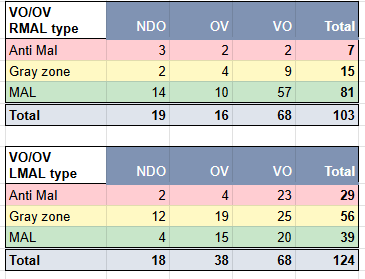
\includegraphics[width=\columnwidth]{latex/HeadRL.png}
\label{tab:FamLR}
\caption{RMAL and LMAL per VO/OV types.}
\end{center}
\end{figure}

In the postverbal domain, we find that VO languages show a more clear bias towards RMAL than OV language. More precisely, out of the 81 languages showing a RMAL effect, that is with a significant positive MAL effect in the postverbal domain, 57 (79\%) are VO, against 10 (12\%) OV languages. Also the anti RMAL preference is particularly rare in VO languages (2 out of 69 languages, 3\%). Inversely, in the preverbal domain, we observe more OV languages with a LMAL preference than VO languages (51\% vs. 38\% of the total of 39 LMAL languages). Importantly, the anti LMAL preference is more frequent in VO languages than in OV languages (79\% vs. 14\% of the total of 29 anti LMAL languages). In other words, one the one hand, VO languages are significantly more likely to show a RMAL preference than OV languages do (84\% vs. 63\%), while they are also less likely to show an anti RMAL preference (3\% vs. 13\%).  On the other hand, OV languages are more likely to show a LMAL preference than VO languages do (39\% vs. 29\%) and they are also less likely to show an anti LMAL preference (11\% vs. 34\%).

These differences are indeed not surprising, given that an asymmetry in terms of the length-based effects is indeed established in the literature between head-final and head-initial languages. They are also in line with previous observations on the difference between the effect of phrasal length in pre- and postverbal domains \citep{faghiriGlossa2020}. We will get back to this in our concluding remarks.


\subsection{MAL compliance in the UD collection}\label{results2}

Out of the total of our 131 languages with a MAL effect, there are 80 with a high MAL compliance, 23 with a low MAL compliance and 28 with a middle MAL compliance (Table \ref{tab:Dec1}. The mean MAL compliance ratio in these three groupes are, respectively, 0.90 (high), 0.13 (low) and 0.50 (middle). This classfication is less strict (precise) and hence results in a smaller number of borderline languages, as well as a greater number of languages at the other side of the cline, with low MAL compliance, compared to Anti MAL languages. But importantly, average decrease ratio values, suggest that both MAL and Anti MAL languages of our sample are well located at the edges of the cline. Based on these observations, We can hence expect the number of Anti MAL languages to increase with a less strict measure and/or classification of the MAL effect.

\begin{figure}[!ht]
\begin{center}
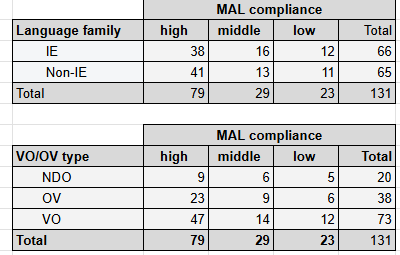
\includegraphics[width=\columnwidth]{latex/Decrease1.png}
\label{tab:Dec1}
\caption{MAL compliance per language families and VO/OV types.}
\end{center}
\end{figure}

Note that we have simliar observations with respect to RMAL and LMAL, which we are not going to present here for the sake of space.
%On the one hand, the MAL preference is stronger in the postverbal domain (about 80\% of the 103 languages for which we have a reliable RMAL metric - average compliance ratios for the three types are 0.95 (high), 0.18 (low) and 0.52 (middle), with respectively 84, 5 and 14 languages per type). On the other hand, the anti MAL preference is stronger in the preverbal domain (about 40\% of 124 languages for which we have a reliable LMAL metric - average compliance ratios for the three types are 0.91 (high), 0.11 (low) and 0.51 (middle), with respectively 57, 50 and 17 languages per type).
